
\section{Introduction}
\section{Motivation}
\section{Matrix formulation of the problem - 1D interferometer}

Here I intend to use convolution matrices properties to {\it qualitatively} study how ``pseudo-PSF'' vary as a
function of source location. Here I limit myselves to a 1-dimensional
interferometer (scalar only), so that
Convolution matrices are Toeplitz-symetyric (see bellow). In a more
general case, (along my intuition - but should be thought more
carefully), convolution matrices should be block-Toeplitz (each
block is a Toeplitz), while symetricity should still be true. 

\subsection{Remarks on the convolution and linear algebra}

In functional form the convolution theorem can be written as follows:


\def\F{\mathcal{F}}
\def\Fm{\bm{F}}
\def\Gauss{\bm{\mathcal{G}}}
\def\conv{\mathcal{*}}

\begin{alignat}{2}
%\label{eq:Lin}
%\F \left{ a.b\right}=&\F \left{ a\right}.\F \left{b\right}\\
\F \left\{  a.b\right\}=& \F \left\{a\right\}\conv\F \left\{b\right\}
\end{alignat}

Noting the convolution product is linear, we can reexpress the
convolution product and associated theorem asing linear
transformations:

\newcommand{\C}[1]{\bm{\mathcal{C}}_{#1}}
\newcommand{\vv}[1]{\bm{#1}}
\def\one{\bm{1}}


\begin{alignat}{2}
\label{eq:ConvTh}
%\F \left{ a.b\right}=&\F \left{ a\right}.\F \left{b\right}\\
\Fm \vv{A}\vv{b}=& \C{\vv{A}}\Fm \vv{b}
\end{alignat}

\noindent where $\Fm$ is the Fourier operator of size 
$n_{uv}\times n_{lm}$ ($\Fm$ is unitary $\Fm^H\Fm=\one$), $\vv{b}$ is
a vector with size $n_{lm}$. The matrix $\vv{A}$ models the scalar
multiplication of each point in $\vv{b}$, and is therefore diagonal of
size $n_{lm}\times n_{lm}$, and $\C{\vv{A}}$ is the convolution matrix
of size $n_{uv}\times n_{uv}$. There is a bijective relation

\begin{alignat}{2}
\label{eq:ConvTh}
%\F \left{ a.b\right}=&\F \left{ a\right}.\F \left{b\right}\\
\vv{A} \longleftrightarrow \C{\vv{A}}
\end{alignat}
 
\noindent in the sense that a scalar multiplucation defines a convolution
function and conversely. The matrices $\vv{A}$ and $\C{\vv{A}}$ always
have the following properties:

\begin{itemize}
  \item $\vv{A}$ is diagonal

   \item In the 1D case
\begin{itemize}
  \item $\C{\vv{A}}$ is Toeplitz
  \item In addition, for radiointerferometry, because the uv plane is symetric, $\C{\vv{A}}$ is symetric
\end{itemize}

\end{itemize}

The matrix $\C{\vv{A}}$ being Toeplitz, each row $\left[ \C{\vv{A}}
  \right]_l$ with sky coordinate $l$ can be built using a
rolling operator $\Delta_l$ that shifts the first row (the PSF at the field
center for example) to location of row $l$:

\begin{alignat}{2}
\label{eq:ConvTh}
%\F \left{ a.b\right}=&\F \left{ a\right}.\F \left{b\right}\\
\left[ \C{\vv{A}} \right]_l =& \Delta_l \left\{ \left[ \C{\vv{A}} \right]_0 \right\}
and&\\
\left[ \C{\vv{A}} \right]_0 =& \Fm^H \ \text{diag}(\vv{A})
\end{alignat}

The rolling operator is essentially just a reindexing, and has the
following properties:

\begin{alignat}{2}
\label{eq:PropsDelta0}
%\F \left{ a.b\right}=&\F \left{ a\right}.\F \left{b\right}\\
\Delta_l \left\{ a\vv{x} \right\} =&  a \Delta_l \left\{\vv{x} \right\} \\
\label{eq:PropsDelta1}
\Delta_l \left\{ \sum_i \vv{x}_i \right\} =& \sum_i \Delta_l \left\{ \vv{x}_i \right\} 
\end{alignat}

\newcommand{\roll}[1]{\Delta_l \left\{#1\right\}}


\subsection{PSF behaviour}

If $\vv{X}$ is the true sky, then the dirty image $\vv{X}^D_{ij}$ of
baseline $(ij)$ can be written as:

\begin{alignat}{2}
\vv{x}^D_{ij} =& \Fm^H \vv{S}_{c,ij}  \C{\vv{T}} \vv{S}_{\square,ij} \Fm \vv{A} \vv{x}
\end{alignat}

\noindent where $\vv{A}_{ij}$ models the DDE effets and is an
$n_{pix}\times n_{pix}$ diagonal matrix (taking polarisation into
account it is an
$4n_{pix}\times 4n_{pix}$ block diagonal matrix), $\vv{T}$ is the tapering/averaging function, 
$\vv{S}_{\square}$ samples the region over which the
tapering/averaging is made, and $\vv{S}_{c,ij}$ selects the central point
of the averaged/tapered visibility set. Using Eq. \ref{eq:ConvTh}, we have:

\begin{alignat}{2}
\vv{x}^D_{ij} =&\ \C{\vv{S}_{c,ij}}  \vv{T} \C{\vv{S}_{\square,ij}}  \Fm^H \Fm \vv{A}_{ij} \vv{x}\\ 
 =&\  \C{\vv{S}_{c,ij}}  \vv{T} \C{\vv{S}_{\square,ij}}  \vv{A}_{ij}  \vv{x}\\ 
\label{eq:approx}
 \sim&\  \C{\vv{S}_{c,ij}}  \vv{T}    \vv{A}_{ij} \vv{x}
\end{alignat}

\noindent where Eq. \ref{eq:approx} is true when the support of the
function $T$ is smaller than the sampling domain of
$\vv{S}_{\square}$. 

Averaged over all baselines, the dirty image becomes:

\begin{alignat}{2}
\label{eq:PPSF}
\vv{x}^D =&\bm{\mathcal{C}}_{STA} \vv{x}\\
\text{with }\bm{\mathcal{C}}_{STA}=&\sum_{ij}  \C{\vv{S}_{c,ij}}  \vv{T}    \vv{A}_{ij}
\end{alignat}



\subsection{Deriving the Pseudo-PSF}

\subsubsection{PSF and Pseudo-PSF}

{\bf We can already see that $\C{\vv{S}_{c,ij}}
  \vv{T}    \vv{A}_{ij}$ in Eq. \ref{eq:approx} is NOT Toeplitz anymore
  because each colunm is multiplied by a different value (DDE
  muliplied by the tapering function). The dirty sky is therefore not
  anymore the convolution of the true sky by the psf} {\it ie} the PSF
varies accross the field of view.

\subsubsection{Slow way}

Calculate the psf estimating $\mathcal{C}$ from direct
calculation. Eventually at discrete locations on a grid.


\subsubsection{Quickly deriving the Pseudo-PSF}

This is tricky part. The problem amount to finding any column $l$ of
$\bm{\mathcal{C}}$ on demand. For notation convenience, we merge
$\vv{T}$ and $\vv{A}_{ij}$ together in $\vv{A}_{ij}$. Operator
$\left[\vec{M}\right]_l$ extracts column $l$ from matrix $\vec{M}$,
and using Eq. \ref{eq:PropsDelta0}, \ref{eq:PropsDelta1} and \ref{eq:PPSF}:

\begin{alignat}{2}
\left[\bm{\mathcal{C}}\right]_l =&
     \left[\sum_{ij}  \C{\vv{S}_{c,ij}}  \vv{A}_{ij}\right]_l\\
=& \sum_{ij} a^l_{ij} \left[\C{\vv{S}_{c,ij}}\right]_l \\
&\ \ \ \text{with } a^l_{ij}=\vv{A}_{ij}(l)\\
=& \sum_{ij} \roll{a^l_{ij} \left[\C{\vv{S}_{c,ij}}\right]_0} \\
=& \sum_{ij} \roll{\Fm^H a^l_{ij}\ \text{diag}\left(\vv{S}_{c,ij}\right) }
\end{alignat}

If we now assume that at any given location $l$, the scalar $a^l_{ij}$
can be described by a smooth {\it function} of the uv coordinates
($(ij)$-indices), then we can write:

\begin{alignat}{2}
\left[\bm{\mathcal{C}}\right]_l =
& \sum_{ij} \roll{ \Fm^H \vv{A}^l\ \text{diag}\left(\vv{S}_{c,ij}\right) }\\
=& \sum_{ij} \roll{\C{\vv{A}^l}\ \Fm^H \text{diag}\left(\vv{S}_{c,ij}\right) }\\
=& \sum_{ij} \roll{\C{\vv{A}^l}\ \left[\C{\vv{S}_{c,ij}}\right]_0 }\\
=& \roll{\C{\vv{A}^l}\ \sum_{ij} \left[\C{\vv{S}_{c,ij}}\right]_0 }\\
=& \roll{\C{\vv{A}^l}\ \left[\C{\vv{S}_{c}}\right]_0 }\\
\end{alignat}

The approximate observed Pseudo-PSF is the convolution of the PSF at
the phase center ($\left[\C{\vv{S}_{c}}\right]_0$) and the fourier transform of the uv-dependent tapering function at given
lm ($\C{\vv{A}^l}$).

In other words, to compute the PSF at a given location $(lm)$:

\begin{itemize}
  \item Find $\vv{A}$:
    \begin{itemize}
    \item Compute weight $w_{ij}$ for each baseline $(ij)$
    \item Fit the uv-dependent weight by (for example), a Gaussian function $w_{ij}\sim w(u,v)=\Gauss\left(u,v\right)$ 
    \end{itemize}
  \item Compute the $PSF_{lm}$ at $(lm)$ from the PSF at the phase center $PSF_0$ as $PSF_{lm}=\mathcal{F}^{-1}\left(w\right)\conv PSF_0$
\end{itemize}
For example if the long baselines are more tapered, they are
"attenuated". The effective PSF on the edge of the field will get
larger by the convolution...
Something like that...
\section{Numerical Experiments}
We demonstrate the computational complexity of the quick, the slow derived PSF as a function of sky coordinates and 
perform a direct numerical results.
\subsection{Slow derivation}
\subsection{Quick derivation}
We will now show how to derived a pseudo PSF  which is based and resolved on the nominal PSF
but labelled by a set of band-limited integration.
\subsubsection{Averaging case}
In order to further optimize the slow derivation of the PSF described above for particularly reduce the computational
cost, we will need to understand the concepts and theory of signals correlation in aperture synthesis.
It is worth noting in Radio Astronomy community that the cross-correlator output of two elements interferometer
in response to a source with spectral brightness distribution $I_{\nu}(\mathbf{s})$ as a function of the pointing direction $\mathbf{s}$ 
is the visibility function defined in Eq.\ref{eq:1} and obtained by integrating
over the solid angle $d\Omega$ (see Thomson, annnff, ahhhh, jjdkk)
\begin{alignat}{2}
V_{\nu}(\mathbf{b}) =& \int_{\Omega}I_{\nu}(\mathbf{s})e^{\frac{-2\pi\nu i \mathbf{b}\mathbf{s}}{c}}d\Omega, \label{eq:1}
\end{alignat}
where $\mathbf{b}$  is the so called "\textit{baseline vector}" with module the distance between the two elements
interferometer and $c$ is the speed of the light. The measurement in Eq.\ref{eq:1} is over the entire 
surface of the celestial sphere, in practice the measurement is generally taken over a finite surface erea of 
the celestial sphere due to the  
finite nature of the tracking source and other effects. Assuming that the frequency $\nu$ and the 
time $t$ change small  enough so that $I_{\nu}(\mathbf{s})$
remains constant while the complex phase, $\frac{-2\pi\nu i \mathbf{b}\mathbf{s}}{c}$ varies linearly.   Eq.\ref{eq:1} becomes:
\begin{alignat}{2}
V_{\nu}(\mathbf{b}) =& \frac{1}{\Delta t \Delta \nu}\int_{\Delta \nu}^{}\int_{\Delta t}^{}\bigg[\int\limits_{\Omega}^{}I_{\nu}(\mathbf{s})e^{\frac{-2\pi\nu i \mathbf{b}\mathbf{s}}{c}} d\Omega\bigg] dt d\nu \label{eq:2}\\	    
		    =& \iint\limits_{-\infty}^{\hspace{.3cm}+\infty}f_{\mathbf{s}}(\mathbf{b})\bigg[\int\limits_{\Omega}^{}I_{\nu}(\mathbf{s})e^{\frac{-2\pi\nu i \mathbf{b}\mathbf{s}}{c}}d\Omega \bigg]dt d\nu  \label{eq:3}.
\end{alignat}
Here, $f_{\mathbf{s}}(\mathbf{b})$ is the visibilities plane tapering funtion, theoretically it is an elliptical function that
mapped the ellipse formed by the baseline.
Eq.\ref{eq:3} allows us to completely understand that in theory, we integrated over a continue elliptical arc both
in frequency and time. 
For convenient and in the rest of this paper, Eq.\ref{eq:3} is restricted to the complex visibility
measured by the two elements interferometer for a point source locates toward the direction 
$\mathbf{s}$ with unitary brightness. A delay correction by the among of $\frac{\mathbf{b}\mathbf{s_0}}{c}$ is generally applied to the signals from the 
array antennas to steer the array toward the direction $\mathbf{s_0}$.
Therefore, the scalar product $\frac{\nu \mathbf{b}(\mathbf{s}-\mathbf{s_0})}{c}=u_{t\nu}l + v_{t\nu}m + w_{t\nu}(\sqrt{1-l^2 - m^2}-1)$
described the time deference between the two incoming signals. Note that
$u_{t\nu}, v_{t\nu}, w_{t\nu}$ are the components of  $\mathbf{b}$ 
given in wavelength and $l,m, \sqrt{1-l^2-m^2}-1$ are the components of  $\mathbf{s}-\mathbf{s_0}$ given in radian, describing the 
three directions cosine. 
We can write:
\begin{alignat}{2}
V_{\nu}(\mathbf{b})  =& \iint\limits_{-\infty}^{\hspace{.3cm}+\infty}f_{lm}(u_{t\nu},v_{t\nu})e^{-2\pi i (u_{t\nu}l+v_{t\nu}m+w_{t\nu}(n-1))}dt d\nu\\
		      =& \check{f}_{lm}(u_{t\nu},v_{t\nu})\circ \delta(u_{t\nu},v_{t\nu}) \label{eq:4}
\end{alignat} %\iint\limits_{\inf}^{\inf}
Where $\check{f}_{lm}$ is the Fourier transform of $f_{lm}$.
In practice, the variation is limited to a small finite frequency range, $\Delta \nu$ centered at $\nu_c$ 
and time range $\Delta t$ centered
at $t_c$, which implies that we are not more integrating over continues elliptical arcs but on shorts discrete
segments across time and frequency. In this case,  $f_{lm}(u_{t\nu},v_{t\nu})$ is troncated over a box, $\Pi_{lm}(u_{t\nu},v_{t\nu})$ 
of size $\Delta t \times \Delta \nu$.
Let supose that $f^{\Pi}_{lm}(u_{t\nu},v_{t\nu})=\Pi_{lm}(u_{t\nu},v_{t\nu})w(u_{t\nu},v_{t\nu})f^{}_{lm}(u_{t\nu},v_{t\nu})$ is 
the troncated version of  $f_{lm}(u_{t\nu},v_{t\nu})$ including a weighting function $w(u_{t\nu},v_{t\nu})$.
We have: %thus over a square taper. Eq.\ref{eq:4} becomes:
\begin{alignat*}{2}
V_{\nu}(\mathbf{b}) =& \check{f}^{\Pi}_{lm}(u_{t\nu},v_{t\nu})\circ\delta(u_{t\nu},v_{t\nu})\\
					 %=& \frac{1}{\Delta \nu \Delta t}\int_{\nu_c - \frac{\Delta \nu}{2}}^{\nu_c + \frac{\Delta \nu}{2}}\int_{t_c - \frac{\Delta t}{2}}^{t_c + \frac{\Delta t}{2}}
%e^{-2\pi i (u_{t\nu}l+v_{t\nu}m+w_{t\nu}(n-1))} dt d\nu\\
		    =& \Bigg[\check{\Pi}_{lm}(u_{t\nu},v_{t\nu})\circ \check{w}(u_{t\nu},v_{t\nu})\circ \check{f}^{}_{lm}(u_{t\nu},v_{t\nu})\Bigg]\circ \delta(u_{t\nu},v_{t\nu})\\
		    =&\Bigg[sinc\frac{-2\pi t\Delta \nu}{2}sinc\frac{-2\pi\nu\Delta t}{2}e^{-2\pi i (u_{t_c\nu_c}l+v_{t_c\nu_c}m+w_{t_c\nu_c}(n-1))}\Bigg]
\end{alignat*}			
\begin{alignat}{2}				 
		     \hspace{1.2cm}\circ \check{w}(u_{t\nu},v_{t\nu})\circ \check{f}^{}_{lm}(u_{t\nu},v_{t\nu})\circ\delta(u_{t\nu},v_{t\nu})\label{eq:5} 
\end{alignat}
It is then observed that for finite frequency and time range, the complex phase varies linearly within the range
$\Delta \Phi = −2\pi t\Delta \nu$ and $\Delta \Psi= −2\pi\nu\Delta t$ in frequency and time respectively.


O.M. Smirnov (cite, Jan 2011) demonstrated that in the case of averaging, natural weighting where
$f^{\Pi}_{lm}(u_{t\nu},v_{t\nu})=\Pi_{lm}(u_{t\nu},v_{t\nu})$, the bove Equation is approximated in term of the
phase changes in time $\Delta \Psi$ and frequency  $\Delta \Phi$ for the case
of smearing as:
\begin{alignat*}{2}
V_{\nu}(\mathbf{b})^{\Pi}_{t_c \nu_c} &\simeq sinc\frac{\Delta \Psi}{2}sinc\frac{\Delta \Phi}{2}e^{-2\pi i (u_{t_c\nu_c}l+v_{t_c\nu_c}m+w_{t_c\nu_c}(n-1))}
\end{alignat*}
\begin{alignat}{2}
				      &\circ \delta(u_{t_c\nu_c},v_{t_c\nu_c})\label{eq:6},
\end{alignat}
with,
\begin{alignat*}{2}
\Delta \Psi =&2\pi \Big[(u_{t_s\nu_c}-u_{t_e\nu_c})l + (v_{t_s\nu_c}-v_{t_e\nu_c})m\\
	    & +(w_{t_s\nu_c}-w_{t_e\nu_c})(n-1)\Big]\\
\Delta \Phi =&2\pi \Big[(u_{t_c\nu_s}-u_{t_c\nu_e})l + (v_{t_c\nu_s}-v_{t_c\nu_e})m\\
	    & +(w_{t_c\nu_s}-w_{t_c\nu_e})(n-1)\Big]
\end{alignat*}
where $t_s$, $t_e$, $\nu_s$ and $\nu_e$ are the starting time range, ending time range, starting frequency range and ending frequency
range respectively.
We then generalized the approximation of smearing for a
random taper $f_{lm}(u_{t\nu},v_{t\nu})$ as follows:
\begin{alignat*}{2}
V_{\nu}(\mathbf{b})^{window}_{t_c \nu_c} &\simeq \Bigg[sinc\frac{\Delta \Psi}{2}sinc\frac{\Delta \Phi}{2}e^{-2\pi i (u_{t_c\nu_c}l+v_{t_c\nu_c}m+w_{t_c\nu_c}(n-1))}\Bigg]
\end{alignat*}
\begin{alignat}{2}
					  & \circ \check{w}(u_{t_c\nu_c},v_{t_c\nu_c})\circ \check{f}_{lm}(u_{t_c\nu_c},v_{t_c\nu_c})\circ \delta(u_{t_c\nu_c},v_{t_c\nu_c})\label{eq:5}.
\end{alignat}
Assuming that all the baselines are pointing at the same phase tracking centre, during conventional interferometric imaging,
the baseline visibilities are mapped on a uv-plane, and the result is inverse Fourier transformed:
\begin{alignat}{2}
PSF(\mathbf{s}) \simeq & \mathcal{F}^{-1}\Bigg\{\sum_{i=1,j=1}^{n_v\times n_{bl}}V_{\nu}(\mathbf{b})^{window}_{t_i \nu_j}\Bigg\}\\
		\simeq & C(\mathbf{s})PSF(\mathbf{s_0}),
\end{alignat}
where $PSF(\mathbf{s}_0)$ is the PSF at the phase tracking center
and $C(\mathbf{s})$ is the image plane smearing response for a source
located toward the direction $\mathbf{s}\neq \mathbf{s_0}$, defined as:
\begin{alignat}{2}
C(\mathbf{s}) &= \sum_{i=1,j=1}^{n_v\times n_{bl}}w(u_{t_c\nu_c},v_{t_c\nu_c})f_{lm}(u_{t_c\nu_c},v_{t_c\nu_c})\mathcal{F}^{-1}\Bigg\{sinc\frac{\Delta \Psi}{2}sinc\frac{\Delta \Phi}{2}e^{-2\pi i (u_{t_c\nu_c}l+v_{t_c\nu_c}m+w_{t_c\nu_c}(n-1))}.\Bigg\}
\end{alignat}
Here, $n_v\times n_{bl}$ is the array total number of visibilities with $n_v$ and $n_{bl}$ the number of visibilities per 
baseline after averaging and the number of baselines respectively.


The smeared unnormalized PSF of a source, $PSF(\mathbf{s})$ located toward the
direction $\mathbf{s}$ was derived and shown that it is proportional
to the PSF, $PSF(\mathbf{s}_0)$ of a source at the phase centre.
% \begin{figure*}
% 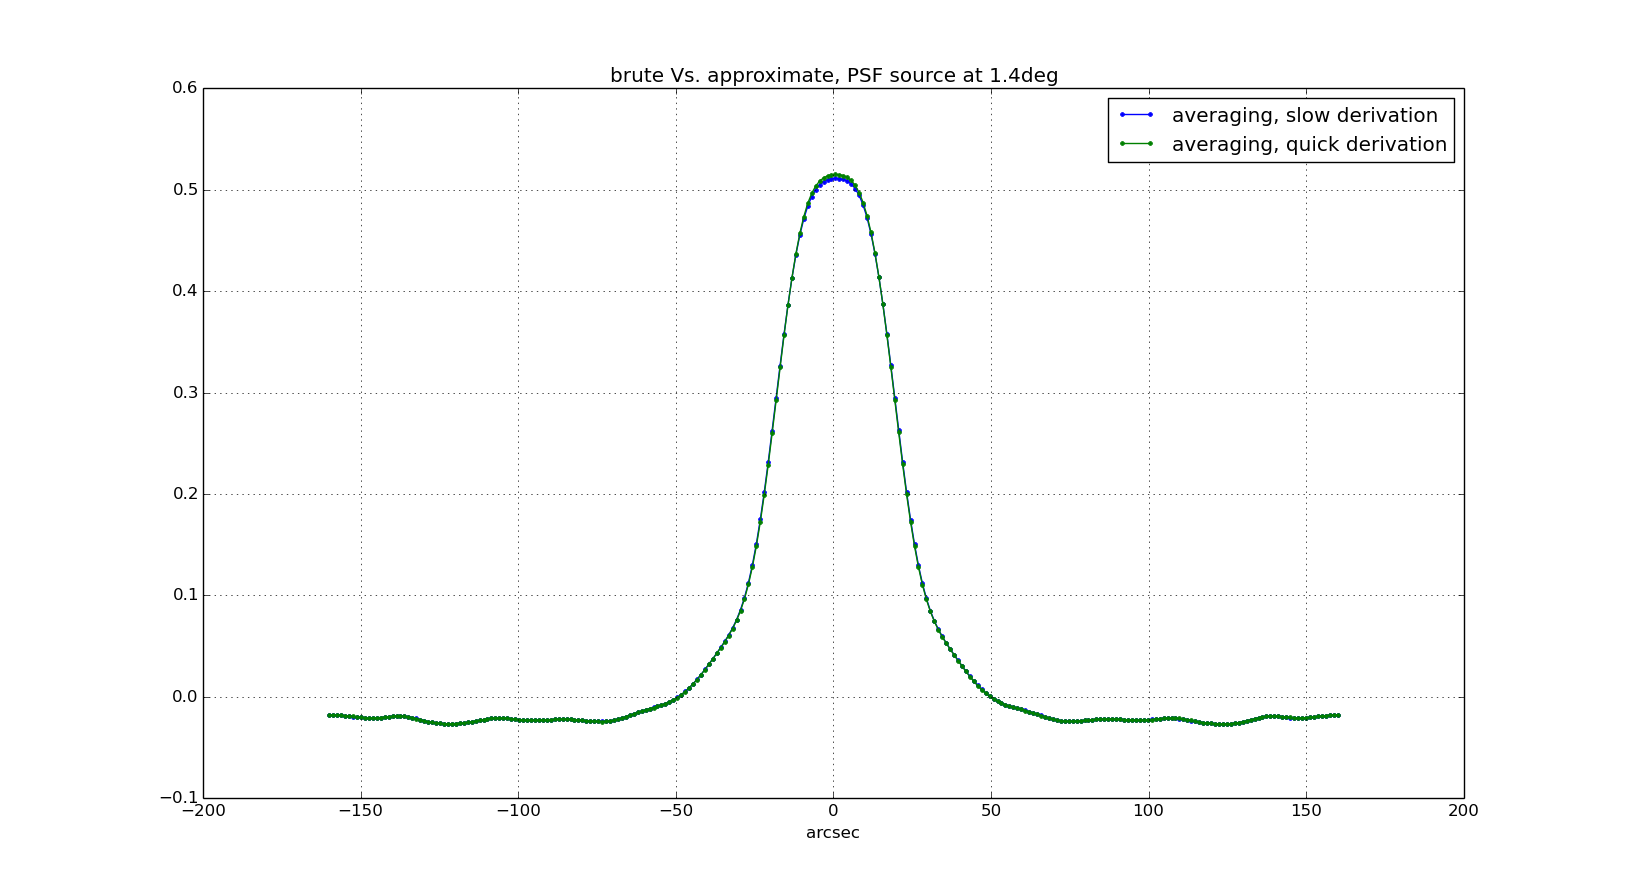
\includegraphics[width=1\textwidth]{./Figures/averaging_brute_quick_good.png}\caption{Brute Vs approximate PSF for a source at 1.4deg}\label{fig:uvcov}
%  \end{figure*}
%  \begin{figure*}
% 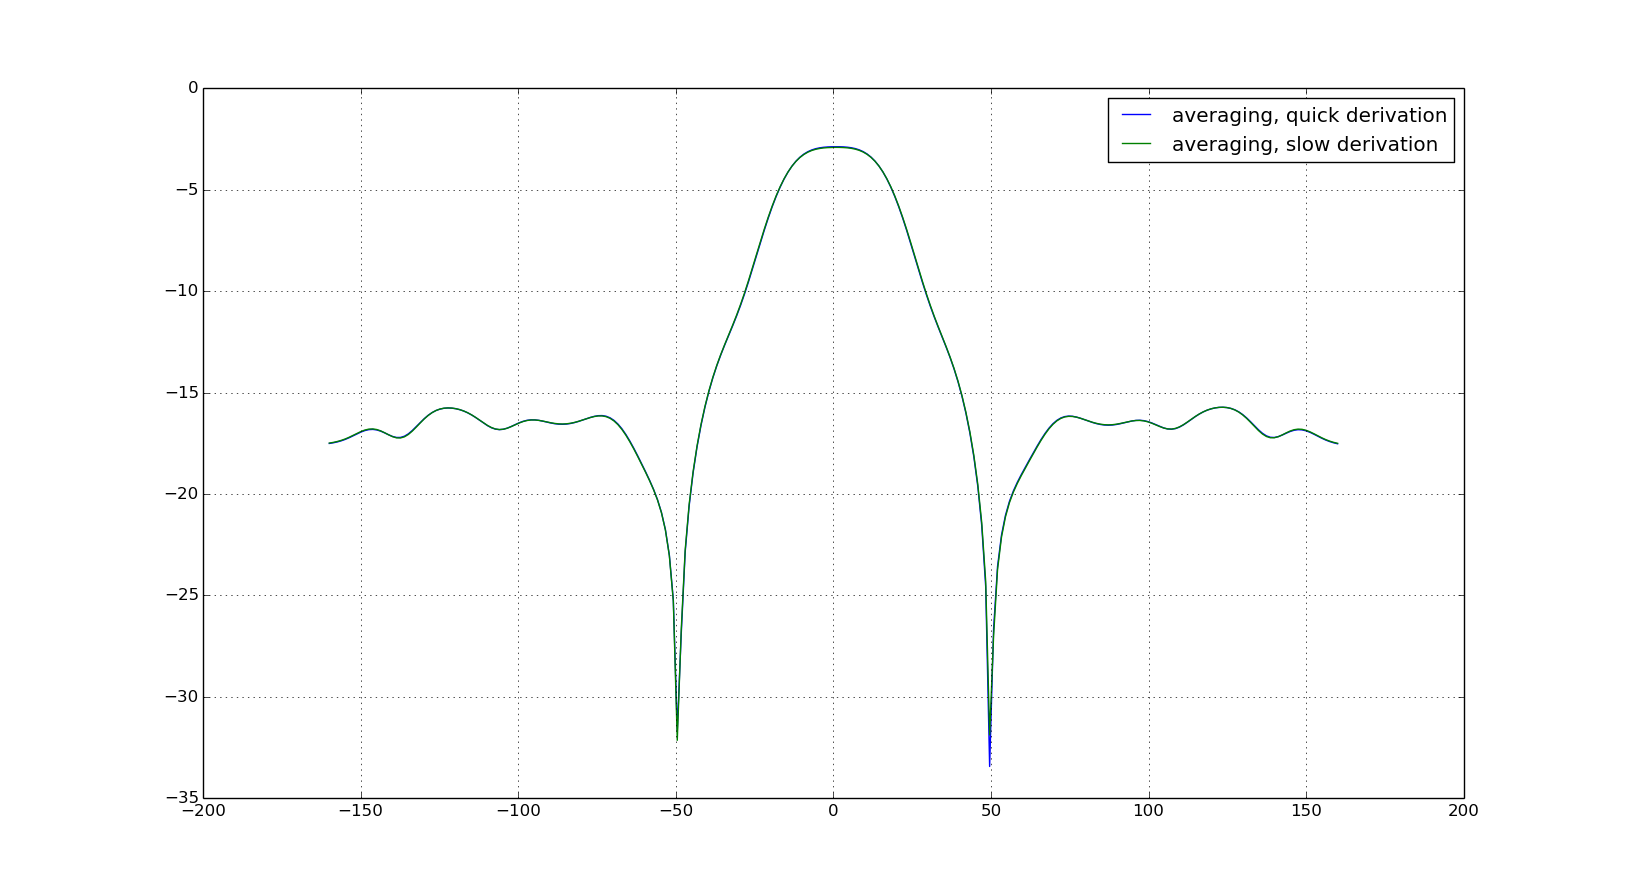
\includegraphics[width=1\textwidth]{./Figures/averaging_brute_quick_logscale.png}\caption{Brute Vs approximate PSF for a source at 1.4deg compare in log space}\label{fig:corrSigVLAMxBl_overlapGdelta}
% \end{figure*}
%  \begin{figure*}
% 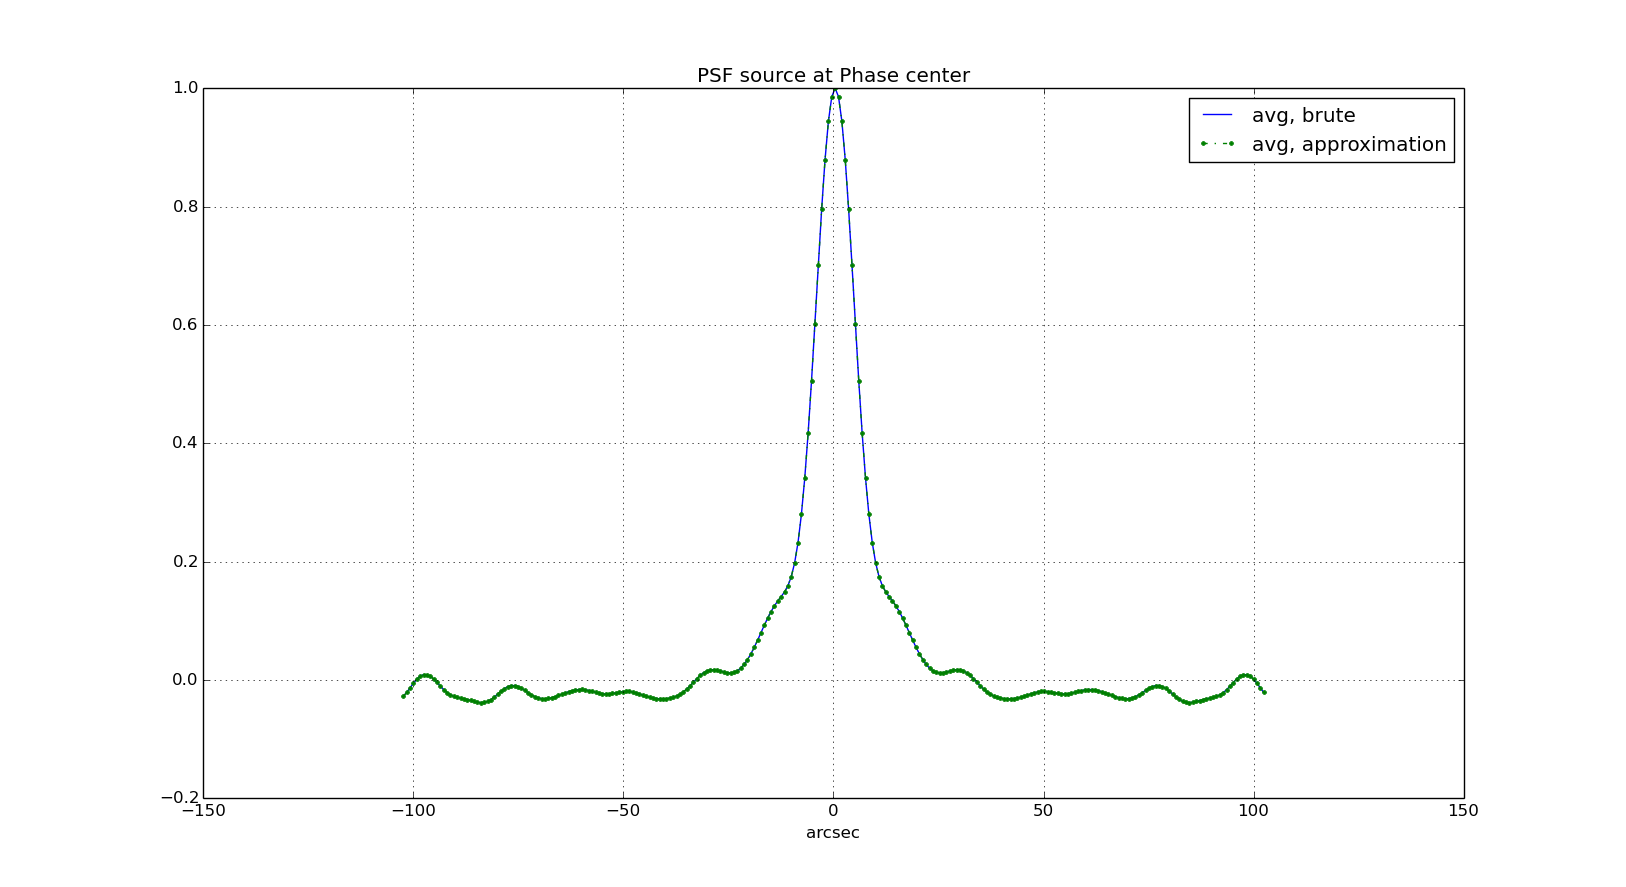
\includegraphics[width=1\textwidth]{./Figures/phasecentre.png}
% \end{figure*}	
% \subsubsection{Computational cost}
% 
% \section{Simulation and comparison}
% \section{Discussion and conclusion}